\section{Motivation}
\subsection{The physics}
\begin{frame}{}{}
	\begin{columns}
	 	\column{.3\textwidth}
	 		\begin{center} 
				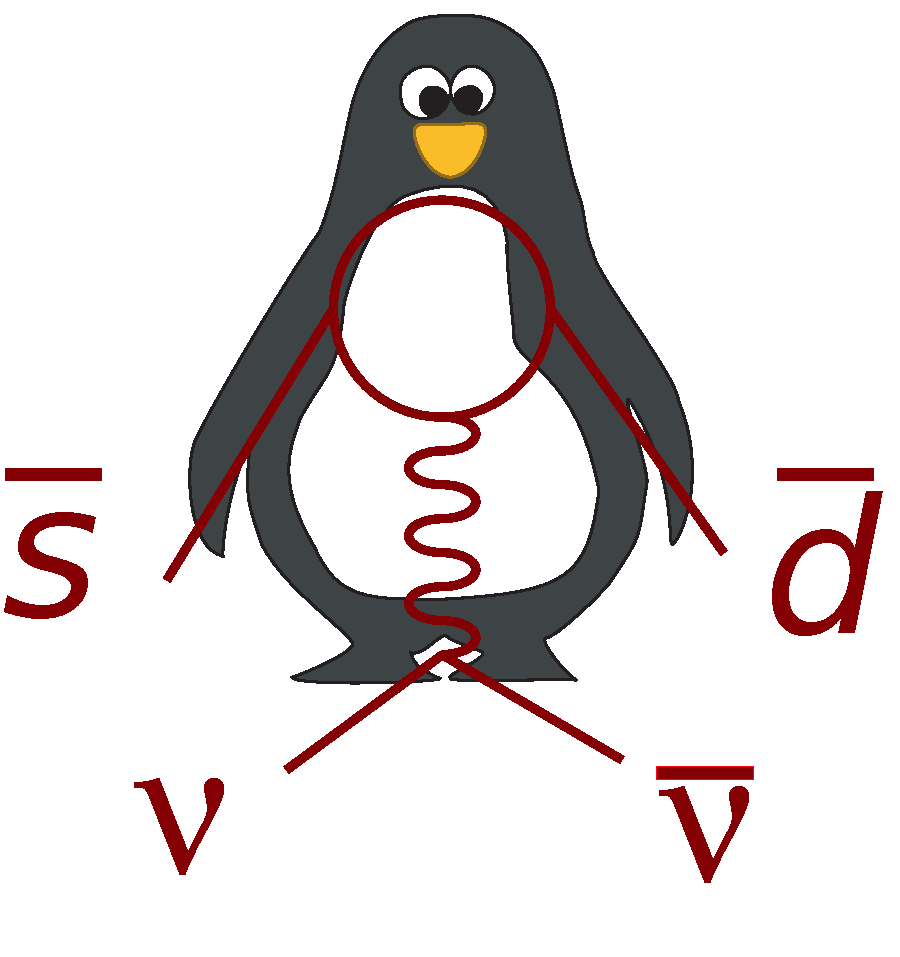
\includegraphics[height=4cm]{penguino}
			\end{center}
	    \column{.65	\textwidth}
	    	\begin{block}{$K^+ \rightarrow \pi^+ \nu \bar{\nu} ~\Leftrightarrow ~
	    	V_{td}$ of CKM matrix} SM branching ratio: $(8.5\pm 0.7)\cdot 10^{-11}$
			\end{block}
			\begin{exampleblock}{NA62 aims $\sigma < 10\%$ with 100 events}
	    		$\approx 10^{13} ~ K^+$ decays required
			\end{exampleblock}
			Data taking planned for 2014-2015, first test run this year 
	\end{columns}
	\begin{block}{Signal-to-noise ratio of 1/10 planned with an event rate of 10
	MHz}
		High efficiency needed $\Rightarrow$ high data rate \\
		\begin{ergo}
			High-performance DAQ and Trigger necessary
		\end{ergo}
	\end{block}
\end{frame}

\subsection{The experiment}
\begin{frame}{NA62 Experiment at CERN}{}
	\begin{center} 
		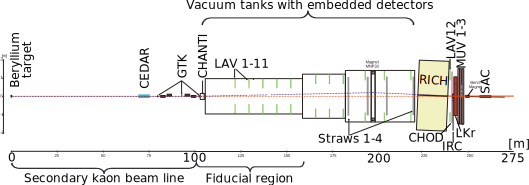
\includegraphics[width=\textwidth]{na62-overview}
	\end{center}
\end{frame}


\begin{frame}{Data rates}{}
	\begin{center}
		\textbf{10 MHz event rate}
	\end{center}
	\begin{table}[H]
		\begin{center}
			\begin{tabular}{c|c|>{\centering\arraybackslash}m{3cm}}
			Detector	&	Event size [B] &	Data rate [GBps]\\
			\hline
			CEDAR	&	216		&	2.16	\\
			GTK 	&	2250	&	22.50 	\\
			CHANTI	&	192		&	1.92 	\\
			LAV 	&	160		&	1.60 	\\
			STRAW 	&	768		&	7.68 	\\
			RICH 	&	160		&	1.60 	\\
			CHOD	&	$\ll1000$	&	$\ll10$\\
			MUV 	&	768		&	7.68 \\
			IRC \& SAC 	& 576	& 	5.76 	\\
			\textbf{LKR}		&	\textbf{222~k}	&	\textbf{2220}	\\
			\hline
			\textbf{Sum}	&	\textbf{$\approx$227~kB}	&	\textbf{$\approx$2.3~TBps}\\
			\end{tabular}
		\end{center}
	\end{table}
\end{frame}